% paper.tex - publication for Monthly Notices of the Royal Astronomical Society

\documentclass[useAMS,usenatbib]{mn2e}
\usepackage{txfonts}
\usepackage{graphicx}
\usepackage{natbib}

\def\del#1{{}}
%\def\del#1{{\bf (DELETED TEXT)}}
%\def\C#1{#1}
\def\C#1{{\bf #1}}

\sloppy

% --- macros --- %
\newcommand{\icm}{intra-cluster medium}
\newcommand{\cmb}{cosmic microwave background}

% --- journals --- %
\newcommand{\aap}{A{\&}A}
\newcommand{\aaps}{A{\&}AS}
\newcommand{\aj}{AJ}
\newcommand{\apj}{ApJ}
\newcommand{\apjl}{ApJL}
\newcommand{\apjs}{ApJS}
\newcommand{\apss}{Ap{\&}SS}
\newcommand{\araa}{ARA{\&}A}
\newcommand{\prd}{Phys. Rev. D}
\newcommand{\pre}{PRE}
\newcommand{\mnras}{MNRAS}
\newcommand{\ssr}{SSRv}
\newcommand{\nat}{Nature}
\newcommand{\physrep}{Phys.~Rep.}
\newcommand{\jcomp}{J.~Comput.~Phys.}

% --- christoph's commands --- %
\newcommand{\dd}{\mathrm{d}}
\newcommand{\bra}{\langle}
\newcommand{\ket}{\rangle}
\newcommand{\ltsima}{$\; \buildrel < \over \sim \;$}
\newcommand{\lsim}{\lower.5ex\hbox{\ltsima}}
\newcommand{\gtsima}{$\; \buildrel > \over \sim \;$}
\newcommand{\gsim}{\lower.5ex\hbox{\gtsima}}
\newcommand{\eps}{\varepsilon}

% --- Anders's commands --- %
\newcommand{\ev}{\mathrm{eV}}
\newcommand{\gev}{\mathrm{GeV}}
\newcommand{\mev}{\mathrm{MeV}}
\newcommand{\tev}{\mathrm{TeV}}
\newcommand{\mpc}{m_{\mathrm{p}}c}
\newcommand{\mpcc}{m_{\mathrm{p}}c^2}
\newcommand{\p}{\mathrm{p}}
\newcommand{\Pp}{\mathrm{P}_\mathrm{p}}
\newcommand{\Pe}{\mathrm{P}_\mathrm{e}}
\newcommand{\pp}{p_\mathrm{p}}
\newcommand{\pe}{p_\mathrm{e}}
\newcommand{\br}{\bold{r}}
\newcommand{\e}{\mathrm{e}}
\newcommand{\ii}{\mathrm{i}}
\newcommand{\inj}{\mathrm{inj}}
\newcommand{\pd}{\partial}
\newcommand{\CR}{\mathrm{CR}}
\newcommand{\gas}{\mathrm{gas}}
\newcommand{\mr}{\mathrm}
\newcommand{\DM}{\mathrm{DM}}
\newcommand{\ISM}{\mathrm{ISM}}
\newcommand{\ICM}{\mathrm{ICM}}
\newcommand{\CMB}{\mathrm{CMB}}
\newcommand{\IC}{\mathrm{IC}}
\newcommand{\mecc}{m_\e c^2}
\newcommand{\mug}{\mathrm{\mu G}}
\newcommand{\rvir}{R_{200}}
\newcommand{\B}{\mathrm{B}}
\newcommand{\ma}{\mathrm{max}}
\newcommand{\low}{\mathrm{low}}
\newcommand{\gae}{\gamma_\mathrm{e}}
\newcommand{\gam}{\gamma}





% --- title --- %
\title{The origin of cosmic-ray electrons in cluster outskirts}

\author[A. Pinzke, P. Oh and C. Pfrommer] 
  {Anders Pinzke$^1$\thanks{e-mail:apinzke@physics.ucsb.edu (AP); peng@physics.ucsb.edu (PO);pfrommer@h-its.org (CP)}, Peng Oh$^1$\footnotemark[1],
    and Christoph Pfrommer$^2$\footnotemark[1]\\
    $^1$University of California - Santa Barbara,
  Department of Physics, CA 93106-9530, USA\\
    $^2$Heidelberg Institute for Theoretical Studies
  (HITS), Schloss-Wolfsbrunnenweg 33, DE - 69118 Heidelberg, Germany}
    

% --- document --- %
\begin{document}
\pagerange{\pageref{firstpage}--\pageref{lastpage}} \pubyear{2011}
\maketitle
\label{firstpage}


% --- abstract --- %
\begin{abstract}
  bla bla bla
\end{abstract}


% --- keywords --- %
\begin{keywords}
  magnetic fields, cosmic rays, radiation mechanisms: non-thermal, elementary
  particles, galaxies: cluster: general
\end{keywords}

% --- section: introduction --- %
\section{Introduction}


\section{Simulations}
\label{sect:simulations}
Our simulations were performed in a $\Lambda$CDM universe using the
cosmological parameters: $\Omega_{\mr m}=\Omega_\DM + \Omega_{\mr
  b}=0.3, \, \Omega_{\mr b}=0.039, \, \Omega_\Lambda=0.7, \, h=0.7, \,
n_{\mr s}=1$, and $\sigma_8=0.9$. The total matter density in units of
the critical density of the universe $\rho_{\rm crit}$ is denoted by
$\Omega_{\mr m}$, the baryonic density by $\Omega_{\mr b}$, the DM
density by $\Omega_\DM$ and the cosmological constant today is denoted
by $\Omega_\Lambda$. The critical density, $\rho_{\rm crit}=3H_0/(8\pi
G)$, where the present day Hubble constant $H_0=100\, h \, \mr{km}\,
\mr{s}^{-1} \, \mr{Myr}^{-1}$. $n_{\mr s}$ represents the spectral
index of the primordial power-spectrum, and $\sigma_8$ denotes the
$rms$ linear mass fluctuation within a sphere of radius $8 \,h^{-1}
\mr{Mpc}$ extrapolated to $z = 0$. The simulations were carried out
with an updated and extended version of the distributed-memory
parallel TreeSPH code GADGET-2 \citep{2005MNRAS.364.1105S,
  2001NewA....6...79S}. Gravitational forces were computed using a
combination of particle-mesh and tree algorithms.  Hydrodynamic forces
are computed with a variant of the smoothed particle hydrodynamics
(SPH) algorithm that conserves energy and entropy where appropriate,
i.e. outside of shocked regions \citep{2002MNRAS.333..649S}.  Our
simulations follow the radiative cooling of the gas, star formation,
supernova feedback, and a photo-ionizing background \citep[details can
  be found in][]{2007MNRAS.378..385P}. We model the cosmic ray (CR)
physics in a self-consistent way \citep{2006MNRAS.367..113P,
  2007A&A...473...41E, 2008A&A...481...33J}.  We include the adiabatic
CR transport process such as compression and rarefaction, and a number
of physical source and sink terms which modify the cosmic ray pressure
of each CR population separately. The most important sources
considered for injection are, diffusive shock acceleration at
cosmological structure formation shocks and shock waves in supernova
remnants, while the primary sinks are thermalization by Coulomb
interactions, and catastrophic losses by hadronization. For
simplicity, in this paper we do not take into account CRs injected
into the inter-stellar medium from supernova remnants (see Pinzke, Oh,
and Pfrommer, in prep. for a discussion of this topic).


\begin{table}
\caption{Cluster sample.}
\begin{tabular}{l l l l r r r}
\hline
\hline
Cluster & sim.'s & dyn. state$^{(1)}$ & $M_{\rm vir}^{(2)}$ & $\rvir^{(2)}$ & $kT_{\rm vir}^{(3)}$ & $\Delta t$$^{(1=4)}$\\
& & & [$\rmn{M}_\odot$] & [Mpc] & [keV] & \\
\hline
1  & g8a  & CC    & $2.6\times 10^{15}$ &   2.9~~ & 13.1 \\
2  & g1a  & CC    & $1.9\times 10^{15}$ &   2.5~~ & 10.6 \\
3  & g72a & PostM & $1.6\times 10^{15}$ &   2.4~~ & 9.4  \\
4  & g51  & CC    & $1.5\times 10^{15}$ &   2.4~~ & 9.4  \\
                                                     
5  & g1b  & M     & $5.2\times 10^{14}$ &   1.7~~ & 4.7  \\
6  & g72b & M     & $2.2\times 10^{14}$ &   1.2~~ & 2.4  \\
7  & g1c  & M     & $2.0\times 10^{14}$ &   1.2~~ & 2.3  \\
8  & g8b  & M     & $1.5\times 10^{14}$ &   1.1~~ & 1.9  \\
9  & g1d  & M     & $1.3\times 10^{14}$ &   1.0~~ & 1.7  \\
                                                     
10 & g676 & CC    & $1.3\times 10^{14}$ &   1.0~~ & 1.7  \\
11 & g914 & CC    & $1.2\times 10^{14}$ &   1.0~~ & 1.6  \\
12 & g1e  & M     & $9.1\times 10^{13}$ &  0.93   & 1.3  \\
13 & g8c  & M     & $8.5\times 10^{13}$ &  0.91   & 1.3  \\
14 & g8d  & PreM  & $7.8\times 10^{13}$ &  0.88   & 1.2  \\
\hline
\end{tabular}  \begin{quote}
 Notes:\\ (1) The dynamical state has been classified through a combined
 criterion invoking a merger tree study and the visual inspection of the X-ray
 brightness maps. The labels for the clusters are M--merger, PostM--post
 merger (slightly elongated X-ray contours, weak cool core (CC) region developing),
 PreM--pre-merger (sub-cluster already within the virial radius), CC--cool
 core cluster with extended cooling region (smooth X-ray profile).  (2) The
 virial mass and radius are related by $M_\Delta(z) = \frac{4}{3} \pi\,
 \Delta\, \rho_\rmn{crit}(z) R_\Delta^3 $, where $\Delta=200$ denotes a
 multiple of the critical overdensity $\rho_\rmn{crit}(z) = 3 H (z)^2/ (8\pi
 G)$.  (3) The virial temperature is defined by $kT_{\rm vir} = G M_{\rm vir} \,
 \mu\, m_\p / (2 R_{\rm vir})$, where $\mu$ denotes the mean molecular weight.
\end{quote}
\label{tab:cluster_sample}
\end{table}



INSERT CLUSTER TABLE WITH DELTA T HERE, USE 100 MYR, AND THE LOG A 

\subsection{CR protons}
For each SPH fluid element we attach a distribution function of CR protons. It is represented by a one-dimensional isotropic distribution function \footnote{The three dimensional distibution function is given by $4\pi \int f(p) p^ 2 \dd p$.} given by
\begin{equation}
  \label{eq:f_p}
  f_\p(p_\p) = \frac{\dd^2 N_\p}{\dd p_\p\,\dd V} = 
  C\, p_\p^{-\alpha}\,\theta(p_\p-q)\,, 
\end{equation}
and $p_\p = P_\p/m_\p c$, where we have normalized the proton momentum
$P_\p$ with the proton mass $m_\p$.  Here $q$ is the mass normalized
momentum cutoff, $\alpha$ the spectral index, and $C$ the
normalization of the distribution function in units of density. 

\del{From our simulated galaxy clusters we derive for each snapshot at time
$t$ the injected CR proton distribution function $f_\p$. We select
particles in the outskirts of clusters where the gas densities are low
and hence the Coulomb cooling of the CR protons small. }

The CR proton
distribution function from the simulations is convinently parameterized in terms of
adiabatic invariant momentum cutoff $q_0$ and the adiabatic invariant
Lagrangian amplitude of the spectrum $\tilde{C}_0$. We convert the adiabatic invariant quantities to physical quantities through
\begin{equation}
  \label{eq:q0}
  q=\left(\frac{\rho}{\rho_0}\right)^{\frac{1}{3}}q_0\,,
\end{equation}
and
\begin{equation}
  \label{eq:C0}
  \tilde{C}=\left(\frac{\rho}{\rho_0}\right)^{-\frac{\alpha-1}{3}}\tilde{C}_0\,,
\end{equation}
where the convenient unitless redefinition of the CR proton amplitude
is given by
\begin{equation}
  \label{eq:Ct}
  \tilde{C}=C\,m_\p/\rho\,.
\end{equation}

From our simulated galaxy clusters we derive for each snapshot at time
$t$ a CR proton distribution function $f_\p$. 

\del{We select
particles in the outskirts of clusters where the gas densities are low
and hence the Coulomb cooling of the CR protons small.}

The injected distribution function is calculated as the change in
CR normalization between a snapshot at time $t$ and an earlier time 
$t-\Delta t$:
\begin{eqnarray}
  \label{eq:finj}
f_\rmn{inj,p}(t,p_\p) &=& \Delta C(t)\,\frac{\rho}{m_\p}\,\rmn{AD(\rho)} \,p_\p^{-\alpha}\qquad\rmn{where}\\
  \Delta  C(t) &=& C(t) - C(t-\Delta t)\,
\end{eqnarray}
and the adiabatic cooling term $\rmn{AD}(\rho)\equiv\left(\rho/\rho_0\right)^{-1/3}$.

We fix the time between each snapshot $\Delta t$ to $100$~Myrs, which
is smaller then the loss timescale of CR electrons in cluster
outskirts. 

\del{The CR proton number density is given by
\begin{equation}
  \label{eq:ncr}
  n_{\CR} = \int_0^\infty \dd p_\p\, f_\p(p_\p) =
  \frac{C\, q^{1-\alpha}}{\alpha-1}\,,
\end{equation}
provided $\alpha >1$. The kinetic energy density of the CR
proton population is
\begin{eqnarray}
  \label{eq:epscr}
  \eps_\CR &=& \int_0^\infty  \dd p_\p\, f_\p(p_\p) \,T_{\rmn
    p}(p_\p)=\frac{C\, m_\p\,c^2}{\alpha-1} \, \times
  \nonumber \\
  && \left[\frac{1}{2}
    \, \B_{\frac{1}{1+q^2}} \left(
    \frac{\alpha-2}{2},\frac{3-\alpha}{2}\right) + q^{1-\alpha}
    \left(\sqrt{1+q^2}-1 \right) \right] \,,
\end{eqnarray}
where $T_\p(p_\p) = (\sqrt{1+p_\p^2} -1)\, m_\p\,c^2$ is the kinetic energy
of a CR proton. $\B_x(a,b)$ denotes the incomplete Beta-function, and
$\alpha>2$ is assumed.}


\section{Radio relics}
\label{section:relics}
RELICS...  Collisionless cluster shocks are able to accelerate ions
and electrons in the high-energy tail of their Maxwellian distribution
functions through diffusive shock acceleration \citep[for reviews
  see][]{1983RPPh...46..973D, 1987PhR...154....1B,
  2001RPPh...64..429M}. Neglecting non-linear shock acceleration and
cosmic ray modified shock structure, then electrons and protons are
indistinguishable in the process of diffusive shock
acceleration. There are, however, difference in: (1) the maximum
energy of the steady state spectrum that depends on the details of the
shock, (2) acceleration efficiency that is related to the smaller
Larmor radius of the electrons that keeps the electrons from diffusing
back and forth over the discontinuity of the shock front.CHECK

In this section we derive the CR electron distribution function by
rescaling the injected CR proton spectrum to account for the different
acceleration efficiencies as well as the shift in momentum due to the
factor $\sim 2000$ difference in mass. In addition we model the
Coulomb and radiative losses of the CR electrons.

\subsection{CR electron distribution function} 
In a hot plasma the temperatures of electrons and protons (ions) are
equal. Under this constraint we derive the relationship between CR
electron momentum and CR proton momentum given by
%\begin{eqnarray}
%  \label{eq:pe_pp}
%\dd \Pe = \dd \Pp \frac{\sqrt{\Pe^2+2\left(m_\e c\right)^2-2m_\e m_\p\,c^2
%+2\left(m_\p-m_\e\right)c\sqrt{\left(m_\e c\right)^2+\Pe^2}}}{\Pe+\left(m_\p-m_\e\right) c \frac{\Pe}{\sqrt{\left(m_\e c\right)^2+\Pe^2}}}
%\end{eqnarray}
\begin{eqnarray}
  \label{eq:pe_pp}
\dd \pe &=& \dd \pp \,g(\pe) =  \dd \pp \,h(\pp)\,,\qquad \rmn{where}\\
g(\pe) &=& X \,\frac{\left[\pe^2-2\left(X-1\right)\left(1-\sqrt{1+\pe^2}\right)\right]^{0.5}}{\displaystyle\pe+\left(X-1\right)\frac{\pe}{\sqrt{1+\pe^2}}}\,,\qquad \rmn{and}\\
h(\pp) &=& X \,\frac{\displaystyle\pp-\left(1-Y\right)\frac{\pp}{\sqrt{1+\pp^2}}}{\left[\pp^2+2\left(1-Y\right)\left(1-\sqrt{1+\pp^2}\right)\right]^{0.5}}\,.\\
\end{eqnarray}
Note that $\pe = \Pe/m_\e c$ and $\pp = \Pp/m_\p c$, where we have
normalized the electron momentum $\Pe$ and the proton momentum $\Pp$
with the electron mass $m_\e$ and proton mass $m_\p$, respectively. We
have introduced the mass ratios $X=m_\p/m_\e$ and $Y=m_\e/m_\p$. Also
note that $\dd \Pe\rightarrow \dd \Pp$ in the asymptotic limit where
$\pp\gg 1$, and that $\dd \Pe\rightarrow \sqrt{m_\e / m_\p}\,\dd \Pp$ for
$\pp\ll 1$. 

The injected CR electron distribution function at each time $t$ is
given by
\begin{eqnarray}
  \label{eq:f_inj_e}
  f_\rmn{inj,e}(p_\e) &=&  \frac{\dd^2 N_\rmn{inj,e}}{\dd V \dd p_\e}(p_\e) = 
\frac{\dd^2 N_\rmn{inj,e}}{\dd V \dd p_\p}(p_\e)\frac{1}{g(p_\e)} \nonumber\\
&=& \frac{\dd^2 N_\rmn{inj,p}}{\dd V \dd p_\p}(p_\p)
\left(\frac{p_\e}{p_\p}\right)^{-\alpha}\frac{\eta_\rmn{max,e}}{\eta_\rmn{max,p}}\frac{1}{g(p_\e)} = 
\Delta C\,p_\e^{-\alpha}\frac{\eta_\rmn{max,e}}{\eta_\rmn{max,p}}\frac{1}{g(p_\e)}\,.
 \nonumber\\
&&
\end{eqnarray}
We use that maximal 50\% of the energy available in a shock is
injected into CR protons ($\eta_\rmn{max,p}$) and a factor 10 smaller
efficiency of 5\% for the CR electrons ($\eta_\rmn{max,e}$).

The CR electrons cool through inverse Compton (IC) emission and
Coulomb losses on timescales that are relative short compared to the
dynamical timescale of a cluster. We model these looses analytically
by instantiniuosly injecting a power-law of electrons at time $t_i$
and evolving it to a later time $t$ (for further details see
\citep{1999ApJ...520..529S}). The loss of energy for each particle is
described by
\begin{equation}
\label{eq:d_cool}
\frac{\dd \gam}{\dd t} = - b(\gam,t)\,,
\end{equation}
where the loss function $b(\gam,t)$ is dominated by Coulomb and IC
losses for the energies and gas densities relevant in this work. The
Coulomb losses are given by
\begin{eqnarray}
  \label{eq:b_C}
  b_\rmn{C}(\gam) &=& b_\rmn{C} \gam^2 
  = \frac{3\,\sigma_\rmn{T}\,n_\rmn{el}\,c}{2}
  \left[\ln\left(\frac{m_\e c^2 \sqrt{\gam-1}}{\hbar\,\omega_\rmn{plasma}}\right)\right.\nonumber \\
    &-&\ln(2)\left(\frac{1}{2}+\frac{1}{\gam}\right)+\frac{1}{2}+
    \left.\left(\frac{\gam-1}{4\gam}\right)^2\right]\,.
\end{eqnarray}
Here $\omega_\rmn{plasma} = \sqrt{4\pi e^2 n_\e / m_\e}$ is the plasma
frequency, and $n_\e$ is the number density of free electrons. Since
the Coulomb losses for relativistic electrons is almost independent of
energy (logarithmic), we approximate that $b_\rmn{C}(\gam,t)\approx
b_\rmn{C}(t)$ \footnote{We use a constant energy $\gamma=10^2$ to
  model the very weak dependence of energy, and note that the
  particular value of $\gamma$ does not matter as long as
  $\gamma\gg1$.}. We can now derive the shift in energy $\gam_i$ at
time $t_i$ to energy $\gam$ at time $t$ due to Coulomb cooling by
integrating Eqn.~(\ref{eq:d_cool}):
\begin{eqnarray}
  \label{eq:gamma_low}
  \gam_\low \equiv\int_{t_i}^{t}\dd t b_\rmn{C}(t) = 
  -\int_{\gam_i}^{\gam}\dd \gam' = -(\gam-\gam_i)\,.
\end{eqnarray}
Since we have discrete snapshots in time we can approximate 
\begin{eqnarray}
  \label{eq:gamma_low_sum}
  \gam_\low = \Delta t \sum_j b_\rmn{C}(t_j)\,,
\end{eqnarray}
where the sum includes all snapshots from time $t_i$ to time $t$. We
now continue with the IC losses that are given by
\begin{equation}
  \label{eq:b_IC}
  b_\IC(\gam,z) = b_\IC \gam^2 (1+z)^4
  = \frac{4}{3}\frac{\sigma_\rmn{T}}{m_\e c} U_\rmn{cmb} \gam^2\,.
\end{equation}
Here $\sigma_\rmn{T}= 8\pi e^4/3(m_\e c^2)^2$ is the Thomson cross
section and $U_\rmn{cmb}$ is the energy density of the CMB at redshift
$z=0$. Similarly to the Coulomb cooling we derive the evolution of energy 
of a particle subject to IC losses through
\begin{equation}
  \label{eq:b_IC_evolu}
\frac{\dd \gam}{\gam^2} = -b_\IC (1+z)^4\dd t\,.
\end{equation}
After a time $(t-t_i)$ has elapsed, all the electrons with
energies above $\gam_\ma$ have thermalized, where we derive $\gam_\ma$
through integrating Eqn.~(\ref{eq:b_IC_evolu}) from injected time
$z_i=z(t_i)$ to a later time $z=z(t)$:
\begin{equation}
  \label{eq:b_max}
   \frac{1}{\gam_\ma} \equiv \frac{1}{\gam} - \frac{1}{\gam_i} = 
   \frac{b_\IC}{H_0}\left[\Lambda(z)-\Lambda(z_i)\right]\,.
\end{equation}
Here $\Lambda(z) \approx z + 1.23\,z^2 + 0.50\,z^3 - 0.14\,z^4 -
0.04\,z^5$ in a Lambda CDM universe and
$H_0=h\,\rmn{km}\,\rmn{s}^{-1}\,\rmn{Mpc}^{-1}$ is the Hubble constant.

Given an initial energy $\gam_i$ of an electron at time $t_i$,
Eqn.~(\ref{eq:d_cool}) can be integrated to give the value of $\gam$
at a later time $t$. The differential population density for
relativistic electrons ($\gam_\e \approx p_\e = P_\e/m_\e c$) is then
given by
\begin{eqnarray}
\label{eq:f_evolv}
f_\rmn{inj,e}(\gam,t,t_i) &=& f_\rmn{inj,e}(\gam_i,t_i)
\left.\frac{\partial\gam_i}{\partial\gam}\right|_t\,,\quad \rmn{where} \\
 f_\rmn{inj,e}(\gam_i,t_i) &=& 
f_\rmn{inj,e}(\gam-\Delta\gam_\IC-\Delta\gam_\rmn{C},t_i) \nonumber\\
&=& f_\rmn{inj,e}(\gam+\frac{\gam^2}{\gam_\ma-\gam}+\gam_\low,t_i)\,,\quad \rmn{and} \\
\frac{\partial\gam_i}{\partial\gam} &=& 
\frac{\gam_\ma^2}{\left(\gam_\ma-\gam\right)^2}\,.
\end{eqnarray}
Here we have used that $\Delta\gam_\IC=-\gam_\low$ and
$\Delta\gam_\rmn{C}=\frac{-\gam^2}{\gam_\ma-\gam}$. The total electron
spectrum is derived from the sum of all individually cooled injected
spectra, starting from the time of injection $t_i$ until a later time
$t$,
\begin{eqnarray}
\label{eq:f_sum}
f_\rmn{tot,e}(\gam,t) = \left(\frac{\tilde{\rho}_{gas}(t)}{\rho_0}\right)^{-1/3}\sum_j f_\rmn{inj,e}(\gam,t,t_j)\,.
\end{eqnarray}
Here the comoving gas density factor $\rho_{gas}(t)$ takes care of the
adiabatic gains and losses, where $\rho_0=1$ is a reference density in
GADGET. Also note that the electrons injected at time $t=t_i$ have not
had the time to cool yet. 

We model the final CR electron spectrum as a superposition of five CR
populations, each determined by Eqn.~\ref{eq:f_sum} but with a
different spectral index and injected spectra. 


\subsection{Synchrotron emission}
The process of merging clusters is often very violent where large
amounts of gravitational energy being dissipated in the form of
radiation, increased temperature, turbulence flows and shocks. The two
latter processes are believed to accelerate CRs to high energy, where
especially the distribution function of preexisting CRs is
enhanced. In this section we use the smooth CR electron distribution
derived from a simulated merging cluster in the previous section,
boost it using the details of the shock, and then finally derive the
radio synchrotron emission.

We fit the steady state CR electron distribution function in
Fig.~\ref{fig:e_spec} with two power-laws
\begin{equation}
  f_\rmn{e,fit}(\gam_\e) = C_1\,\gam_\e^{-\alpha_1}
\theta(\gam_\rmn{break}-\gam_\e) 
+ C_2\,\gam_\e^{-\alpha_2}
\theta(\gam_\e-\gam_\rmn{break})\,. 
\label{eq:f_fit}
\end{equation}
The best fit CR electron normalization is given by ${\bf
  C}=(6\times10^{-4},\,10^{7})$, the spectral index by ${\bf
  \alpha}=(3.0,5.5)$, and the energy where the slope changes by
$\gam_\rmn{break}=1.2\times10^4$.

\C{Probably need to calculate the emissivity numerically since there
  is a break in the power-law spectrum. CHECK} We calculate the radio
synchrotron emissivity of the CR electrons using \cite{1979rpa..book.....R}
\begin{equation}
J_0(\nu) \approx \left(\frac{e^2\,\nu_c}{c}\right)\,\sum_i C_i
\gam\left(\frac{3 \alpha_i-1}{12}\right)\,\gam\left(\frac{3 \alpha_i+19}{12}\right)\frac{3^\frac{\alpha_i}{2}}{\alpha_i+1}\,\left(\frac{\nu}{\nu_c}\right)^{\frac{1-\alpha}{2}}\,,
\end{equation}
where the cyclotron frequency is given by
$\nu_c=e\,B\,c/(2\pi\mecc)$. We derive the total emitted power from
the source by integrating the emissivity over the target volume. Here,
we assume that the target volume haw an uniform distribution of the
CR electrons, hence the total power per unit frequency is given by
\begin{equation}
  P_0(\nu) = \rmn{Volume} \times J_0(\nu)\,.
\end{equation}

NEED TO REWRITE The typical size of a large relic is of the order of a
Mpc, while the thickness is only of the order 100~kpc. We assume that
the rather unknown extension of the relic along the line of sight to
be about 500~kpc, where the total radio emitting volume is about
$0.05~\rmn{Mpc}^3$. In addition we assume that the average magnetic
field in the cluster outskirts to be of the order
$B\approx0.1\,\mu$G. The total emitted power at 1.4 PHz of the size
typical for a large radio Relic is then given by
$P_0(1.4\,\rmn{PHz})=9\times10^{22}$~W/Hz. This is about a factor
10-100 smaller than what is typically expected from a relic
\cite{2009A&A...508...75V}. However, this luminosity is boosted by the
shock or turbulence induced during a cluster merger. We follow the
prescription outlined in \cite{2011ApJ...734...18K} to calculate the
boost in radio luminosity due to reacceleration, and find that
$P_2(1.4\,\rmn{PHz})\sim\times10^{25}$~W/Hz in agreement with several
of the relics listed in e.g. \cite{2009A&A...508...75V}.

The steady-state test-particle solution of the downstream CR
distribution can be written as a function of the pre-existing CRs through
\begin{equation}
  f_2(\gae) = q \gae^{-q}\int_{\gam_\rmn{inj}}^\gam \gam'^{q-1}
   f_\rmn{e,fit}(\gam')\dd \gam'\,.
\end{equation}
Here we have neglected the contribution from the injected CRs. The lowest momentum boundary above which particles can cross the shock is given by 
\begin{equation}
\gam_\rmn{inj} \approx 1.17 \frac{u_2}{c}\left(1+\frac{1.07}{\epsilon_B}\right)
\left(\frac{M}{3}\right)^{0.1}\,.
\end{equation}

Spectral index
\begin{equation}
q(M) = \frac{3\left(u_1-v_ A\right)}{u_1-v_A-u_2} = 
\frac{3\sigma\left(1-M_A^{-1}\right)}{\sigma-1-\sigma M_A^{-1}}
\end{equation}
where $u_1$ and $u_2$ are the speed of the flow upstream and
downstream, respectively, in the shock rest frame. The compression
ratio is given by $\sigma=u_1/u_2=\rho_2/\rho_1$, and $M_A=u_1/v_A$ is
the upstream Alfvén Mach number with velocity
$v_A=B_1/\sqrt{4\pi\rho_1}$. We derive the test-particle power-law
slope $q$ as a function of the shock Mach number $M$ with
$\sigma=[(\gam_\rmn{ad}+1)M^2]/[(\gam_\rmn{ad}-1)M^2+2]$, where
adiabatic index $\gam_\rmn{ad}=5/3$, $M_A=M c_s/v_A$, and $ c_s$ the
upstream sound speed.

Enhanced emissivity calculated with
\begin{equation}
\frac{J_2(\nu)}{J_0(\nu)} \approx \left(\frac{B_2^{\left(r-1\right)/2}}{B_0^{\left(\alpha-1\right)/2}}\right) \,\left[\frac{f_2(\gae)}{f_0(\gae)}\right]_{\gae=10^4}\,
\left(\frac{\nu}{280\,\rmn{MHz}}\right)^{\left(\alpha-r\right)/2}\,.
\end{equation}


OUTLINE THE PRESCRIPTION eq7, eq21


\del{Collisionless cluster shocks are able to accelerate ions and
  electrons in the high-energy tail of their Maxwellian distribution
  functions through diffusive shock acceleration \citep[for reviews
    see][]{1983RPPh...46..973D, 1987PhR...154....1B,
    2001RPPh...64..429M}.  Neglecting non-linear shock acceleration
  and cosmic ray modified shock structure, the process of diffusive
  shock acceleration uniquely determines the spectrum of the freshly
  injected relativistic electron population in the post-shock region
  that cools and finally diminishes as a result of loss
  processes. \del{The inverse Compton emitting electron population
    cools on such a short time scale $\tau_\rmn{sync} < 10^8$~yrs
    (compared to the very long dynamical time scale $\tau_\rmn{dyn}
    \sim 1$~Gyr) that we can describe this by instantaneous
    cooling. In this approximation, there is no steady-state electron
    population and we would have to convert the energy from the
    electrons to inverse Compton (IC) and synchrotron
    radiation. Instead, we introduce a virtual electron population
    that lives in the SPH-broadened shock volume only; this is defined
    to be the volume where energy dissipation takes place. Within this
    volume, which is co-moving with the shock, we can use the
    steady-state solution for the distribution function of
    relativistic electrons and we assume no relativistic electrons in
    the post-shock volume, where no energy dissipation occurs. Thus,
    the cooled CR electron equilibrium spectrum can be derived from
    balancing the shock injection with the IC/synchrotron cooling:
    above a GeV it is given by}
\begin{equation}
\label{eq:f_eq}
f_\e(E) = C_\e\, E^{-\alpha_\e}, \quad
C_\e \propto \frac{\rho}
{\eps_B + \eps_\rmn{ph}}
\end{equation}
}

\begin{figure*}
\begin{minipage}{2.0\columnwidth}
  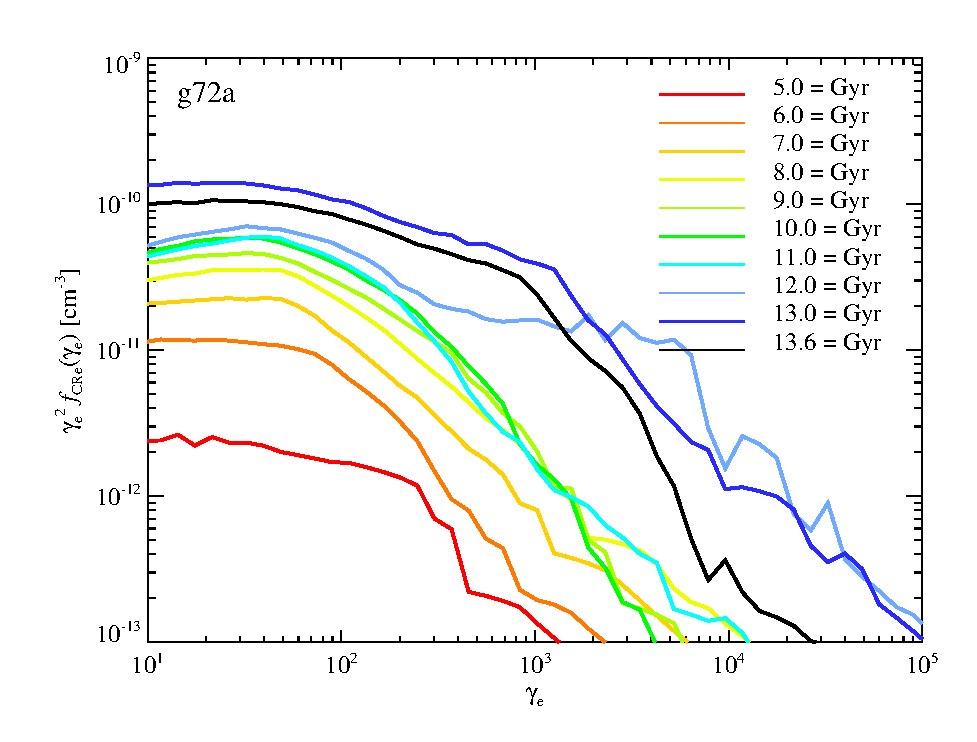
\includegraphics[width=0.32\columnwidth]{./figures/f_z.g72a.1.4Rv.a24.full.v20.eps}
  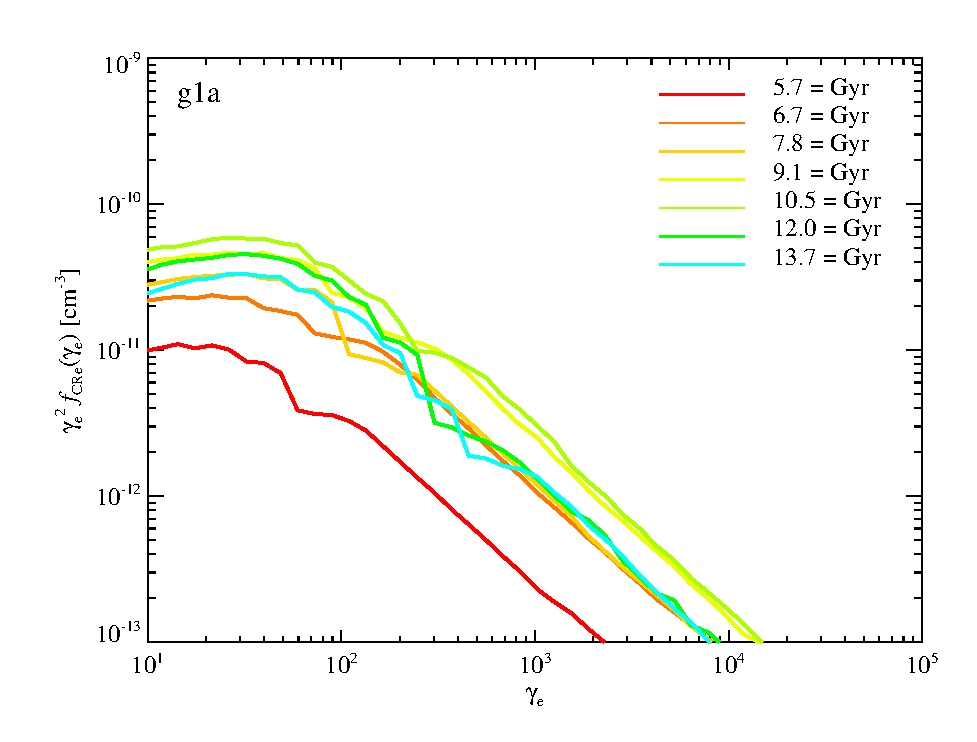
\includegraphics[width=0.32\columnwidth]{./figures/f_z.g1a.1.4Rv.a24.full.v20.eps}
  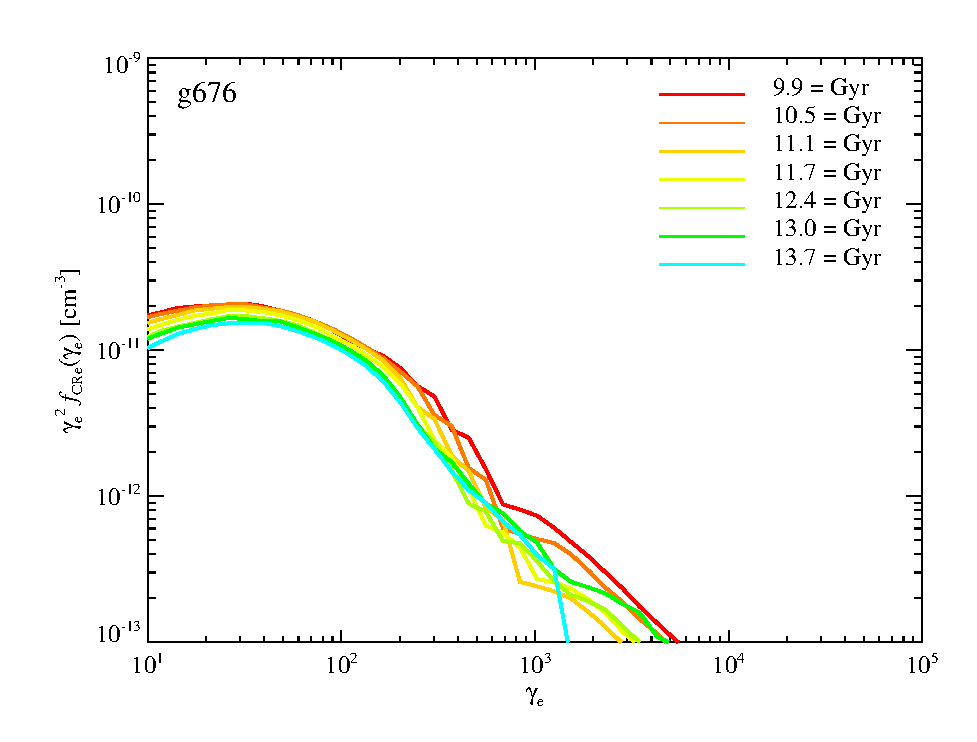
\includegraphics[width=0.32\columnwidth]{./figures/f_z.g676.1.4Rv.a24.full.v20.eps}
  \caption{Time evolution of the cosmic ray electron spectra in
    cluster outskirts. We show the total volume weighted CR electron
    distribution function for the particles that reside end up in
    region between (1.3-1.5)$\rvir$ at redshift zero; a cluster with a
    recent merger (g72a, left panel), large cooling flow cluster (g1a,
    middle panel), and a small cooling flow cluster (g676, right
    panel). The different line colors show the CR electron spectra at
    different look-back times, where the most recent spectrum in black
    is at 13.6 Gyrs. Notice the larger scatter in the merging cluster,
    and the relative small difference in the cooling flow
    clusters. The shape of the distribution function is very similar
    between different cooling flow clusters, and slightly more
    stochastic for merging clusters.\label{fig:e_spec_z}}
\end{minipage}
\end{figure*}

\begin{figure*}
\begin{minipage}{2.0\columnwidth}
  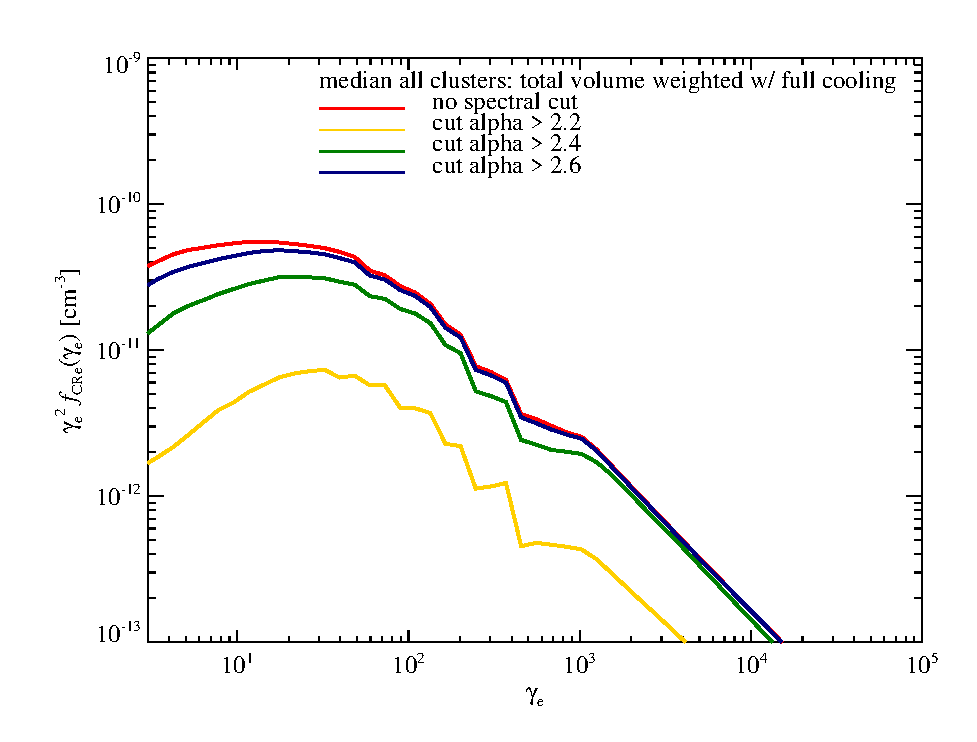
\includegraphics[width=0.49\columnwidth]{./figures/CRspec.alphaCheck.eps}
  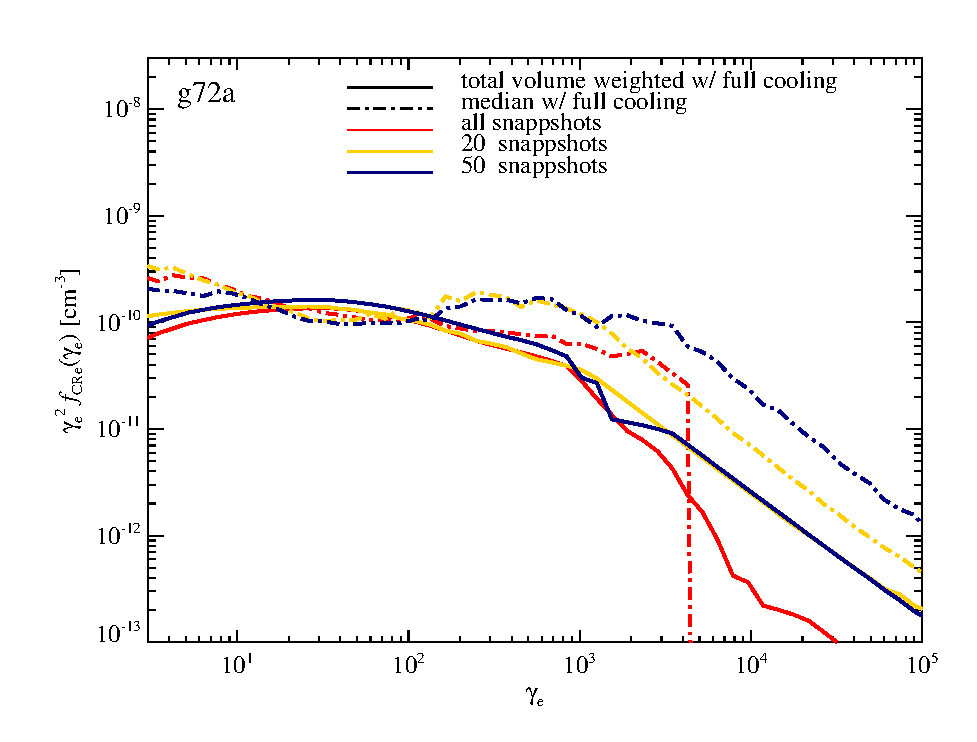
\includegraphics[width=0.49\columnwidth]{./figures/CRspec.snapCheck.eps}
  \caption{Testing the robustness of the CR electron spectra. Left
    panel shows how different cuts in injected spectra impact the
    total volume weighted CR electron spectrum with full cooling; no
    spectral cut (red line), cut particles with $\alpha_\inj>2.2$
    (yellow line), cut particles with $\alpha_\inj>2.4$ (green line),
    cut particles with $\alpha_\inj>2.6$ (blue line). Note that in the
    main CR model we cut all particles with an $\alpha_\inj>2.4$,
    which is a factor four smaller at low energies than the spectrum
    without a cut. Right panel shows the effect of time-resolution on
    the CR electron spectra. The median CR spectrum is shown with full
    cooling that includes radiative, Coulomb, and adiabatic losses
    (dash-dotted line), the solid line represents the total volume
    weighted CR electron spectrum with full cooling. The three line
    colors corresponds to the same cluster, a large coma like merging
    cluster, but with different time resolution between snapshots in
    the relevant regime; red lines corresponds to 100 Myrs between
    snapshots, orange lines corresponds to ~(1.0-1.5) Gyrs between
    snapshots, and the blue lines corresponds to ~(1.0-1.5) Gyrs
    between snapshots. \label{fig:e_spec_tests}}
\end{minipage}
\end{figure*}

\begin{figure*}
\begin{minipage}{2.0\columnwidth}
  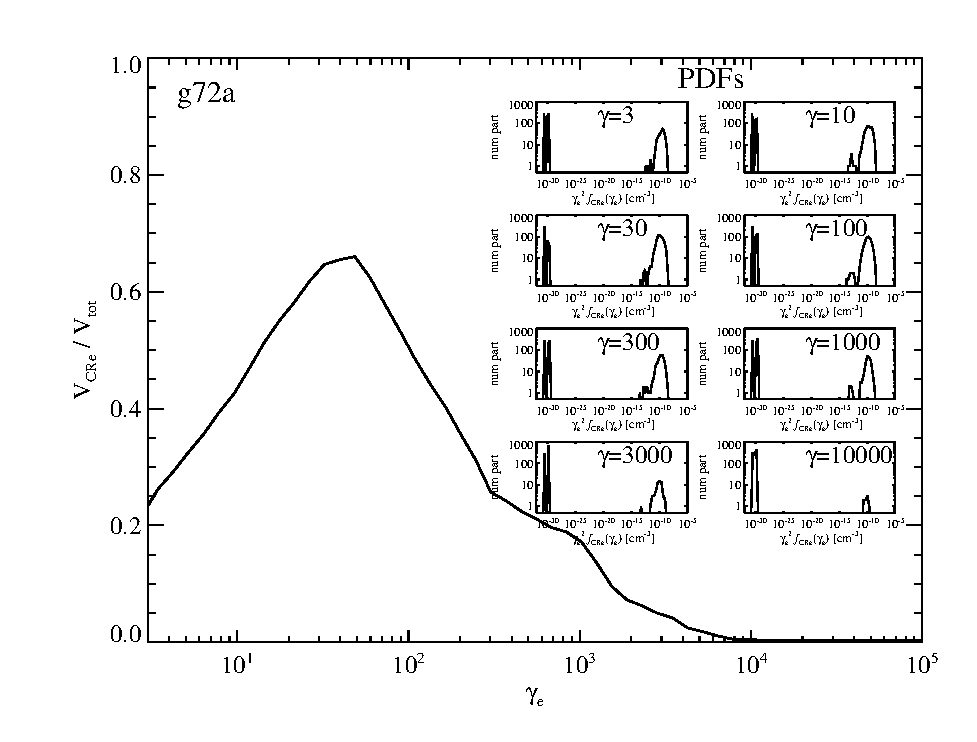
\includegraphics[width=0.49\columnwidth]{./figures/CRvolume.g72a.1.4Rv.a24.full.140.v20.eps}
  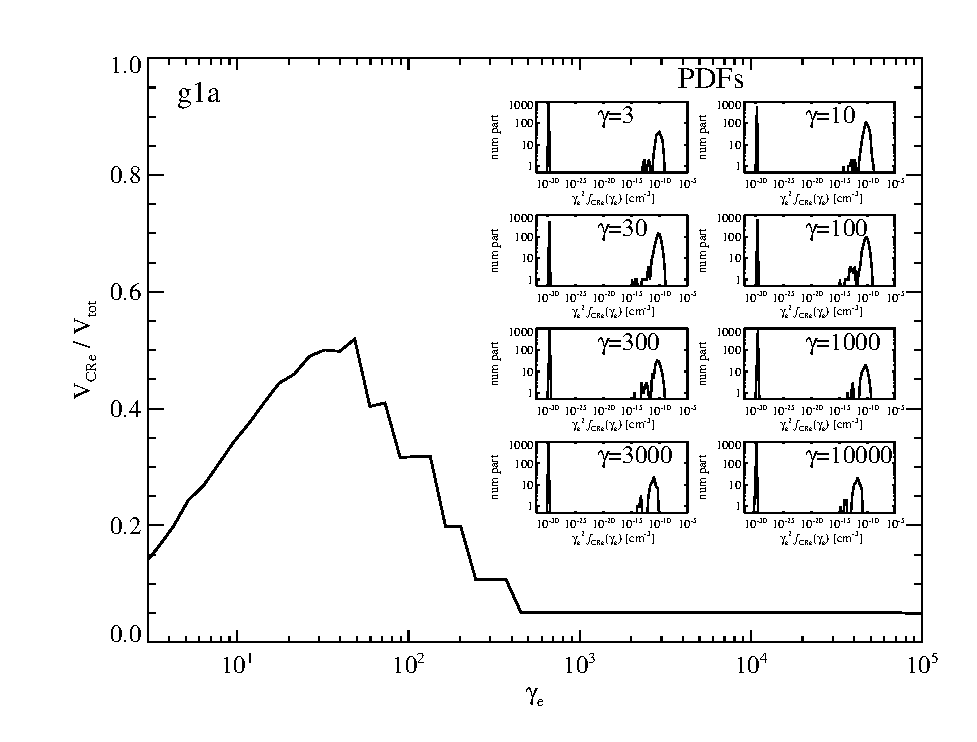
\includegraphics[width=0.49\columnwidth]{./figures/CRvolume.g1a.1.4Rv.a24.full.020.v20.eps}
  \caption{The fractional volume occupied by CR electrons in cluster
    outskirts. Large panels (left Coma like cluster, and right massive
    cooling flow cluster) show the fractional volume occupied by CR
    electrons as a function of logarithmic Lorentz factor ($\gam_\e$)
    in the region between (1.3-1.5)$\rvir$ at redshift zero. The
    smaller panels show the logarithmic particle distribution function
    for different $\gam_\e$, where the left peaks corresponds to
    unpopulated SPH particles and cooled CR particles, while the right
    peaks show the CR populated SPH
    particles. \label{fig:e_spec_CRvolume}}
\end{minipage}
\end{figure*}

\begin{figure}
  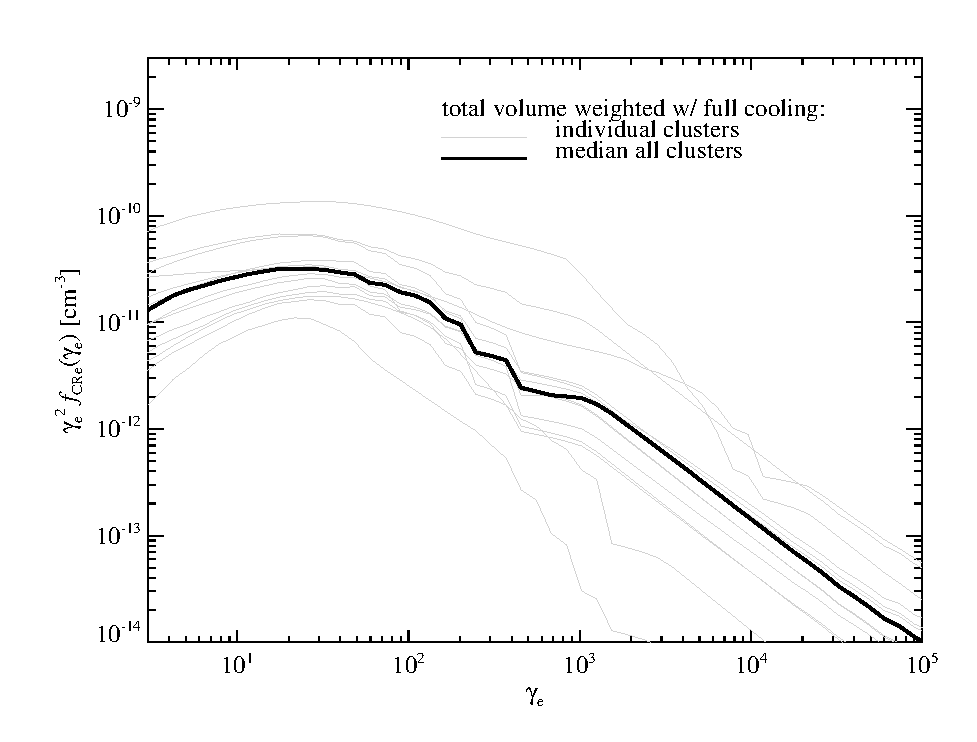
\includegraphics[width=1.0\columnwidth]{./figures/CRespec.all.1.4Rv.a24.full.020.v20.eps}
  \caption{Cosmic ray electron spectra in cluster outskirts at
    redshift zero. We show the total volume weighted CR electron
    distribution function in the region between (1.3-1.5)$\rvir$ with
    full cooling that includes radiative, Coulomb, and adiabatic
    losses. The the thin grey lines show the spectra from individual
    clusters while the thick solid line shows the median of the
    spectra from all clusters. \label{fig:e_spec_all}}
\end{figure}

\begin{figure}
  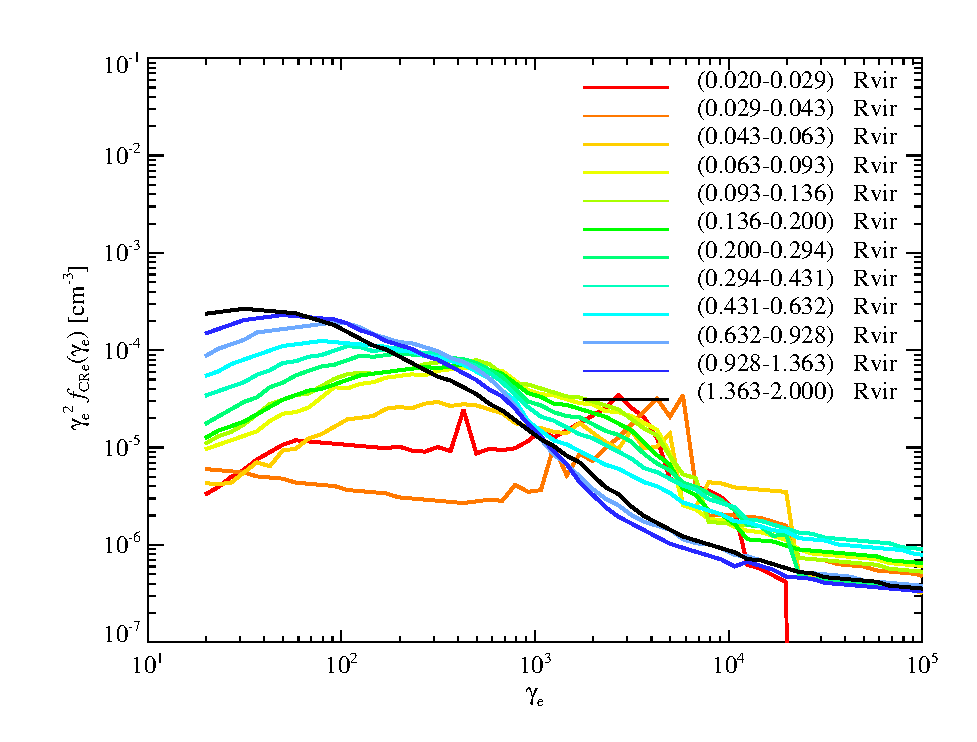
\includegraphics[width=1.0\columnwidth]{./figures/old/CRespecRadial.Radial2Rv.a24.140.v16.eps}
  \caption{Spatial dependence of the cosmic ray electron spectra at
    redshift zero. We show the total volume weighted CR electron
    distribution function; a Coma like cluster (left panel), a massive
    cooling flow cluster (middle panel), and the median of our 14
    cluster's spectra (right panel). The different line colors show
    the CR electron spectra for different radial
    bins.\label{fig:e_spec_spatial}}
\end{figure}

\begin{figure}
  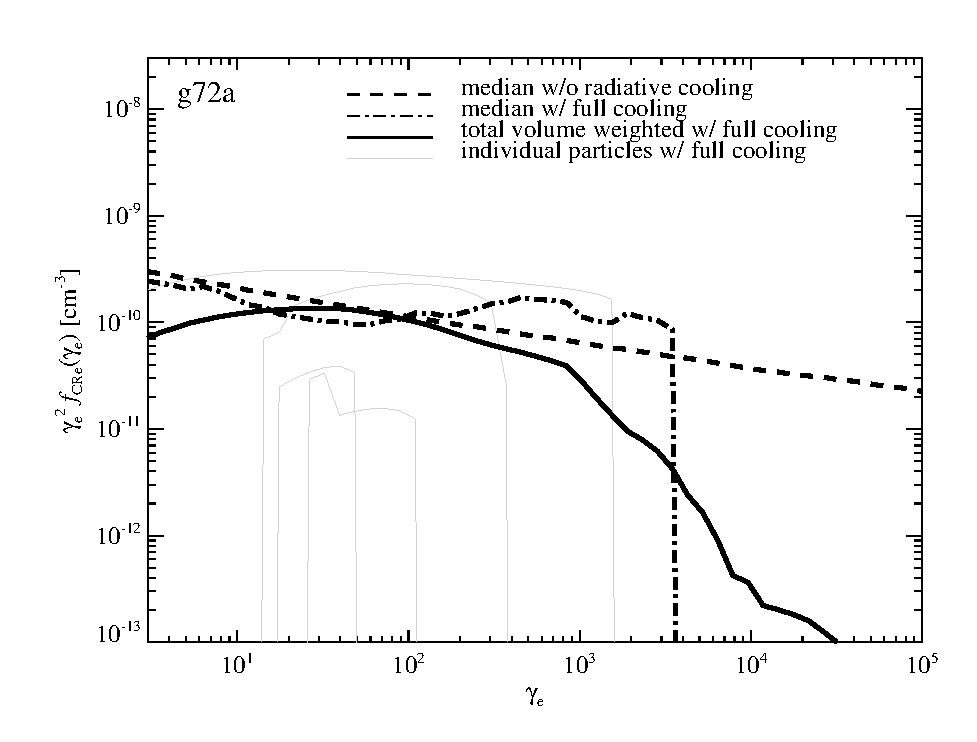
\includegraphics[width=1.0\columnwidth]{./figures/CRespec.g72a.1.4Rv.a24.full.140.v20.eps}
  \caption{Cosmic ray electron spectra in cluster outskirts at
    redshift zero. We show the CR electron distribution function
    weighted with the electron Lorentz factor ($\gam_\e$) squared for
    a typical cluster with a recent merger for region between
    (1.3-1.5)$\rvir$. The median CR spectrum is shown with full
    cooling that includes radiative, Coulomb, and adiabatic losses
    (dash-dotted line), and with only adiabatic losses (dashed
    line). The solid line represents the total volume weighted CR
    electron spectrum with full cooling. Note that the Coulomb cooling
    at low energies is very inefficient because of the low electron
    densities in the cluster outskirts.\label{fig:e_spec_g72a}}
\end{figure}

\del{
\begin{figure*}
\begin{minipage}{2.0\columnwidth}
%  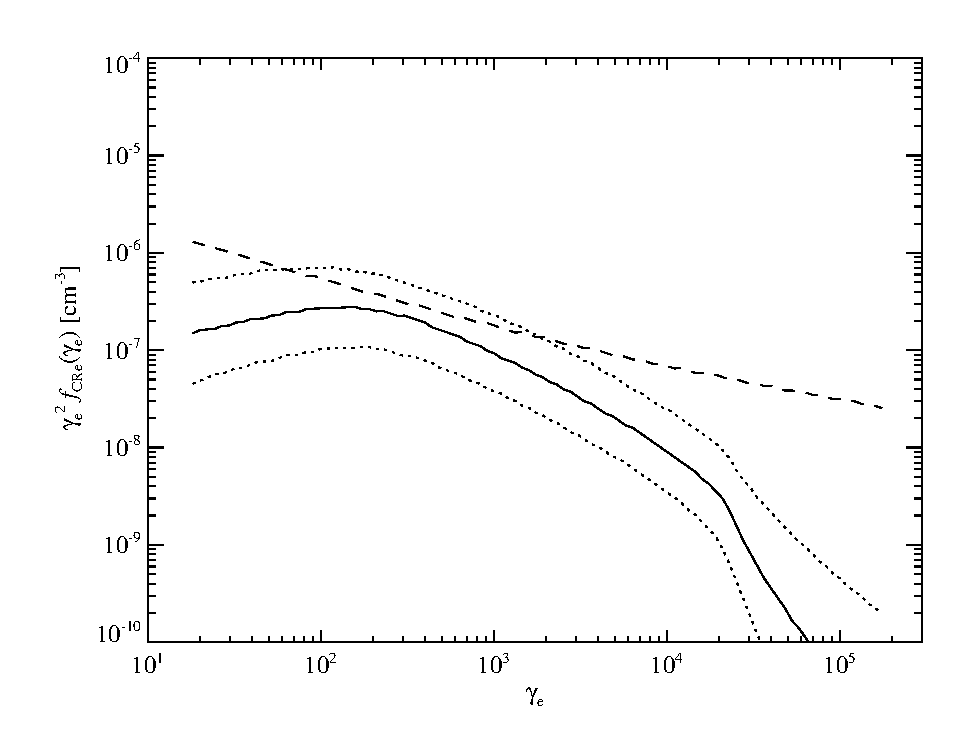
\includegraphics[width=0.49\columnwidth]{./figures/CRespec0.3Rv.140.v12.eps}
%  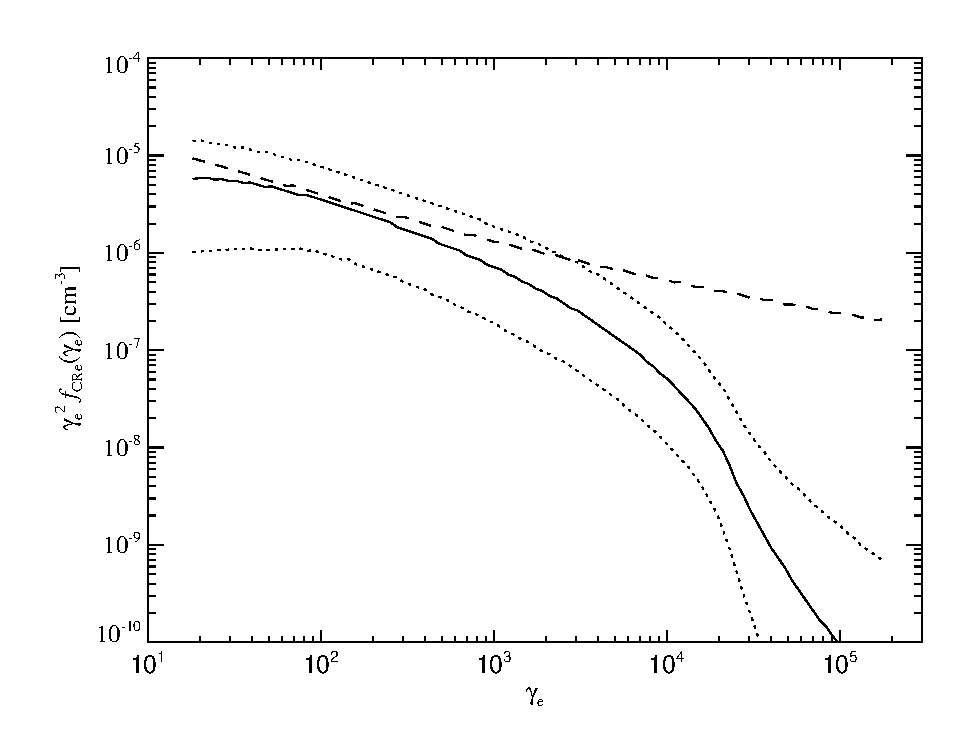
\includegraphics[width=0.49\columnwidth]{./figures/CRespec1.4Rv.140.v12.eps}
  \caption{Cosmic ray electron spectra in cluster outskirts at
    redshift zero. We show the CR electron distribution function
    weighted with the electron Lorentz factor ($\gam_\e$)
    squared. In the {\it left panel} panel we show the CR electron in
    the region between (0.3-0.5)$\rvir$ and in the {\it right panel}
    between (1.3-1.5)$\rvir$. The solid lines show the median CR
    electron spectrum where both radiative and adiabatic losses are
    included. The dotted lines shows the 68 percentiles. The dashed
    lines show the CR electron spectrum without Coulomb and radiative
    cooling. Note that the Coulomb cooling at low energies is very
    inefficient because of the low electron densities in the cluster
    outskirts. \label{fig:e_spec}}
\end{minipage}
\end{figure*}
}

\del{
\begin{figure*}
\begin{minipage}{2.0\columnwidth}
%  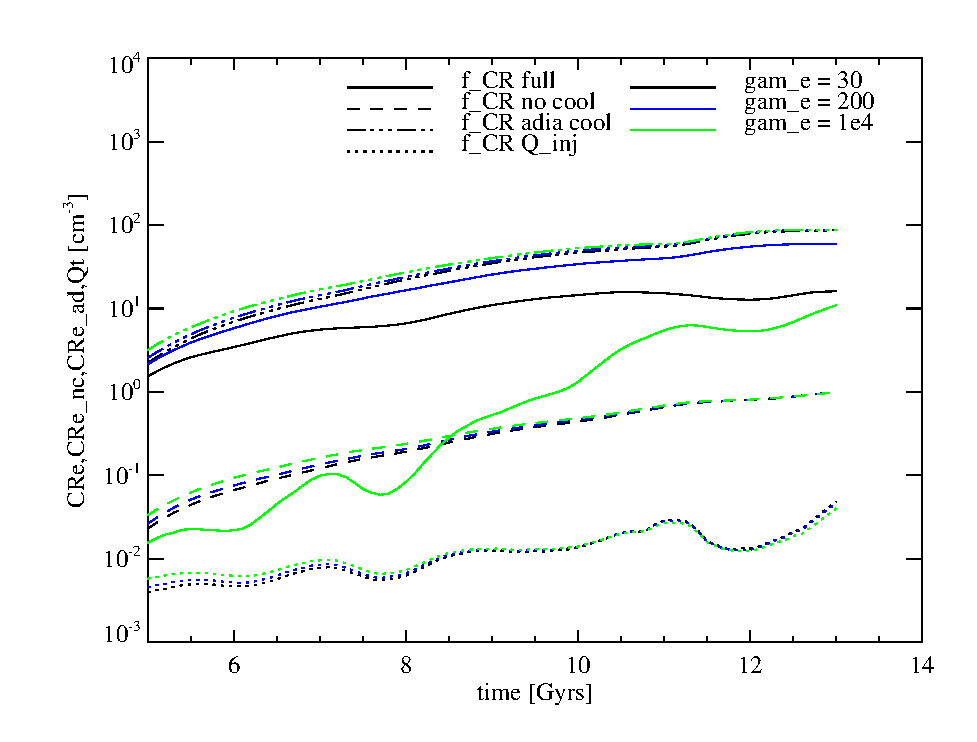
\includegraphics[width=0.49\columnwidth]{./figures/f_evolution.0.3Rv.eps}
%  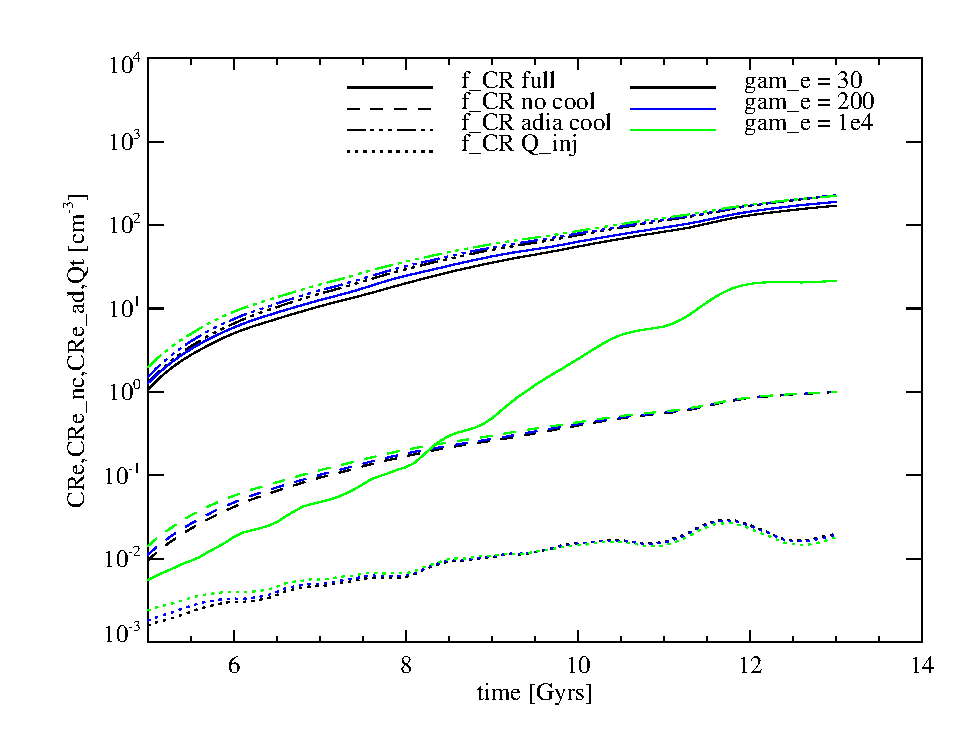
\includegraphics[width=0.49\columnwidth]{./figures/f_evolution.1.4Rv.eps}
  \caption{Time evolution of cosmic ray (CR) electron spectra. We show
    the CR electron distribution function weighted with the electron
    Lorentz factor ($\gam_\e$) squared. The time evolution of the CR
    electrons which at $z=0$ reside from (0.3-0.5)$\rvir$ are shown in
    the {\it left panel} and (1.3-1.5)$\rvir$ in the {\it right
      panel}. The black lines show the CR electrons with a
    $\gam_\e=30$, blue lines $\gam_\e=200$, and green lines
    $\gam_\e=10^4$. The solid lines show the CR electrons with full
    cooling, i.e. for Coulomb, inverse Compton, and adiabatic
    losses. Dashed lines show the CR electrons without Coulomb and
    inverse Compton cooling while the dash-dotted lines show the CR
    electrons without adiabatic cooling. The dotted line show the
    injected CR electron distribution function, derived from the
    injected CR protons. For each energy, we normalize the CR electron
    distribution function with the CR electrons without
    cooling. Notice that the high energy part is built up during the
    last Gyr. This is explained by the inverse Compton losses that are
    larger at high energies, especially at high redshifts where the
    energy density of the CMB is much larger than
    today.  \label{fig:e_evol}}
\end{minipage}
\end{figure*}
}

\del{
\begin{figure*}
\begin{minipage}{2.0\columnwidth}
%  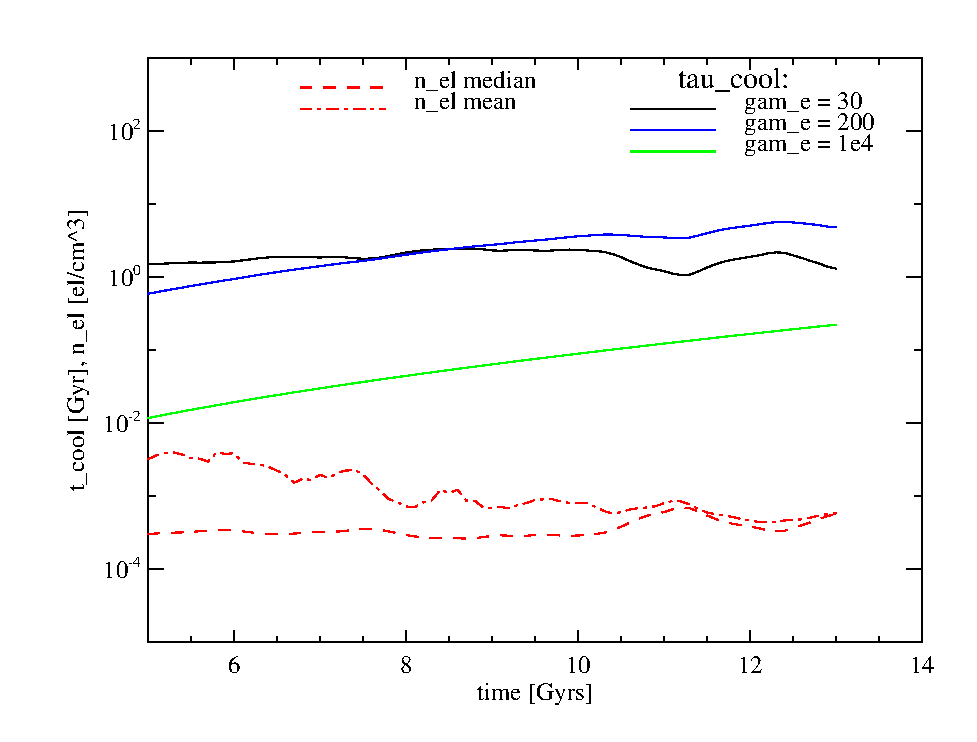
\includegraphics[width=0.49\columnwidth]{./figures/evolution.0.3Rv.eps}
%  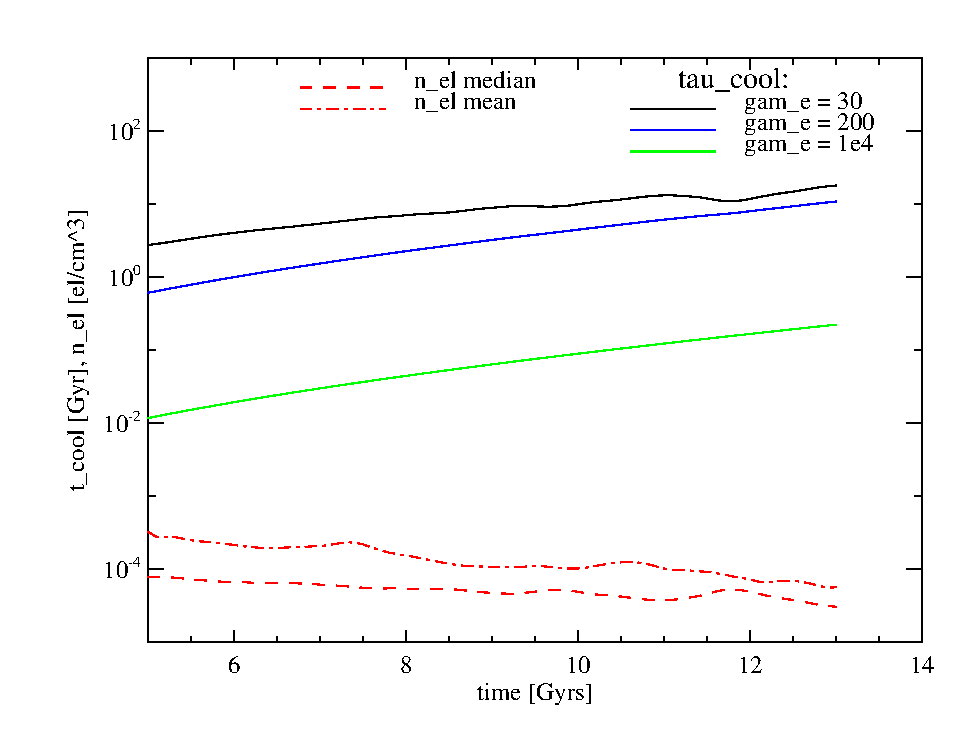
\includegraphics[width=0.49\columnwidth]{./figures/evolution.1.4Rv.eps}
  \caption{Time evolution of the gas density and the cosmic ray (CR)
    cooling time. We show the time evolution of the electron number
    density and CR electron cooling time that are associated with the
    CR electrons which at redshift $z=0$ reside from (0.3-0.5)$\rvir$
    in the {\it left panel} and (1.3-1.5)$\rvir$ in the {\it right
      panel}. The red lines show the electron number densities, where
    the dashed line show the median and dash-dotted the mean. The
    solid lines show the cooling times
    $\tau_\rmn{cool}=\gam_\e/[b_\IC(\gam_\e)+b_\rmn{C}(\gam_\e)]$
    for $\gam_\e=30$ (black), $\gam_\e=200$ (blue), and
    $\gam_\e=10^4$ (green). Interesting the CR cooling at low
    energies of the particles that end up in the center is constant
    while is increasing monotonically for the particles that end up in
    the cluster periphery. The density of the particles that end up in
    the center is roughly constant with time while it is decreasing
    for the particles that end up in the outer part. This is due to
    the expansion of the universe that counteract the contraction of
    the particles in the cluster periphery. \label{fig:evol}}
\end{minipage}
\end{figure*}
}

% --- section: --- %
\section{Conclusions}
\label{sect:conclusions}

% --- section: --- %
\section*{Acknowledgments}

% --- section: bibliography --- %
\bibliography{bibtex/paper}
\bibliographystyle{mn2e}

\appendix

\bsp

\label{lastpage}

\end{document}
